% SchemaForge --- Complete two-page project summary
% Compile: tectonic SchemaForge_Summary.tex
\documentclass[8pt,a4paper]{extarticle}
\usepackage[T1]{fontenc}
\usepackage{lmodern}
\usepackage[margin=1.45cm,top=1.3cm,bottom=1.2cm]{geometry}
\usepackage{booktabs}
\usepackage{enumitem}
\usepackage{xcolor}
\usepackage{titlesec}
\usepackage{tabularx}
\usepackage{multicol}
\usepackage{tikz}
\usetikzlibrary{arrows.meta,positioning,calc}
\usepackage[colorlinks=true,linkcolor=black,urlcolor=sfnavy]{hyperref}
\definecolor{sfnavy}{HTML}{16324F}
\definecolor{sfrule}{HTML}{B8C4D0}
\definecolor{sfbox}{HTML}{F2F5F8}
\definecolor{sfred}{HTML}{A4243B}
\titleformat{\section}{\normalfont\large\bfseries\color{sfnavy}}{}{0pt}{}
\titlespacing*{\section}{0pt}{1.25ex plus .2ex}{0.45ex}
\setlist[itemize]{leftmargin=1.2em,itemsep=0.15ex,topsep=0.25ex}
\setlist[enumerate]{leftmargin=1.5em,itemsep=0.15ex,topsep=0.25ex}
\renewcommand{\arraystretch}{1.08}
\setlength{\parindent}{0pt}
\setlength{\parskip}{0.5ex}
\setlength{\columnsep}{1.1em}
\newcommand{\code}[1]{\texttt{\small #1}}
\tikzset{
  box/.style={draw=sfrule, fill=sfbox, rounded corners=1.6pt, align=center,
              inner xsep=3pt, inner ysep=2.5pt, font=\scriptsize},
  forge/.style={box, draw=sfnavy, fill=sfnavy!8, line width=0.6pt},
  danger/.style={box, draw=sfred, fill=sfred!7, line width=0.6pt},
  store/.style={box, draw=sfnavy!45, fill=white},
  flow/.style={-{Stealth[length=1.5mm]}, draw=sfnavy, line width=0.45pt},
  gated/.style={-{Stealth[length=1.5mm]}, draw=sfred, line width=0.6pt},
  token/.style={-{Stealth[length=1.5mm]}, draw=sfred, line width=0.5pt, dashed},
  lbl/.style={font=\tiny\itshape, text=sfnavy, inner sep=1pt},
  rlbl/.style={font=\tiny\bfseries, text=sfred, inner sep=1pt},
}
\newcommand{\nohyph}{\hyphenpenalty=10000 \exhyphenpenalty=10000 \sloppy}
\pagestyle{empty}

\begin{document}

\begin{center}
  {\color{sfnavy}\LARGE\bfseries SchemaForge}\\[0.5ex]
  {\normalsize Rehearse PostgreSQL migrations, prove what happened, stop before production}\\[0.4ex]
  {\footnotesize TrueFoundry $\times$ Polaris ``Agents That Act'' Hackathon \textperiodcentered\ Complete Project Summary \textperiodcentered\ September 2026}
\end{center}
\vspace{0.1ex}
{\color{sfrule}\hrule height 1pt}
\vspace{0.7ex}

\colorbox{sfbox}{\parbox{\dimexpr\linewidth-2\fboxsep}{\centering\itshape
The model proposes; tools measure; policy constrains; a human decides.}}

\section*{1 \textperiodcentered\ The problem}
Schema migrations are simultaneously the most attractive and the most dangerous job to hand to an AI agent. A model can write plausible DDL in seconds, but \emph{plausible} is not \emph{safe}. A migration that survives code review still fails against real data: a \code{NOT NULL} constraint collides with rows nobody knew were empty, a type change silently truncates, an \code{ACCESS EXCLUSIVE} lock stalls a hot table, or a dropped column takes its data with it. Three things are missing from the naive ``agent writes SQL and runs it'' loop:

\begin{itemize}
  \item \textbf{Evidence.} Nothing has actually executed against representative data, so every claim about duration, locks and row impact is a guess dressed as a fact.
  \item \textbf{Reversibility.} A rollback script that has never been run is a hypothesis, not a plan.
  \item \textbf{A boundary the agent cannot cross.} ``Ask before doing something irreversible'' is a prompt instruction, and prompt instructions are advice, not enforcement.
\end{itemize}

SchemaForge treats all three as engineering problems rather than prompting problems.

\section*{2 \textperiodcentered\ What it is}
A TrueForge agent that converts a natural-language database change into an evidence-backed decision. It inspects a live PostgreSQL~16 target, maps the dependency blast radius, executes the generated SQL inside a rollback-only shadow sandbox, checks explicit assertions and rollback equivalence, and then \textbf{freezes} with a decision packet. Nothing reaches production without a cryptographically signed approval bound to that exact SQL and that exact assertion set, plus a second Allow/Deny gate inside TrueForge. The interesting output is often the refusal.

\section*{3 \textperiodcentered\ Architecture}
Two role-separated MCP servers (TypeScript, Streamable HTTP) attach to one TrueForge agent. The split is structural, not advisory: configuration validation refuses to boot a process holding a credential it should not have, so the model-facing half physically cannot write production or mint an approval.

\begin{center}
\nohyph
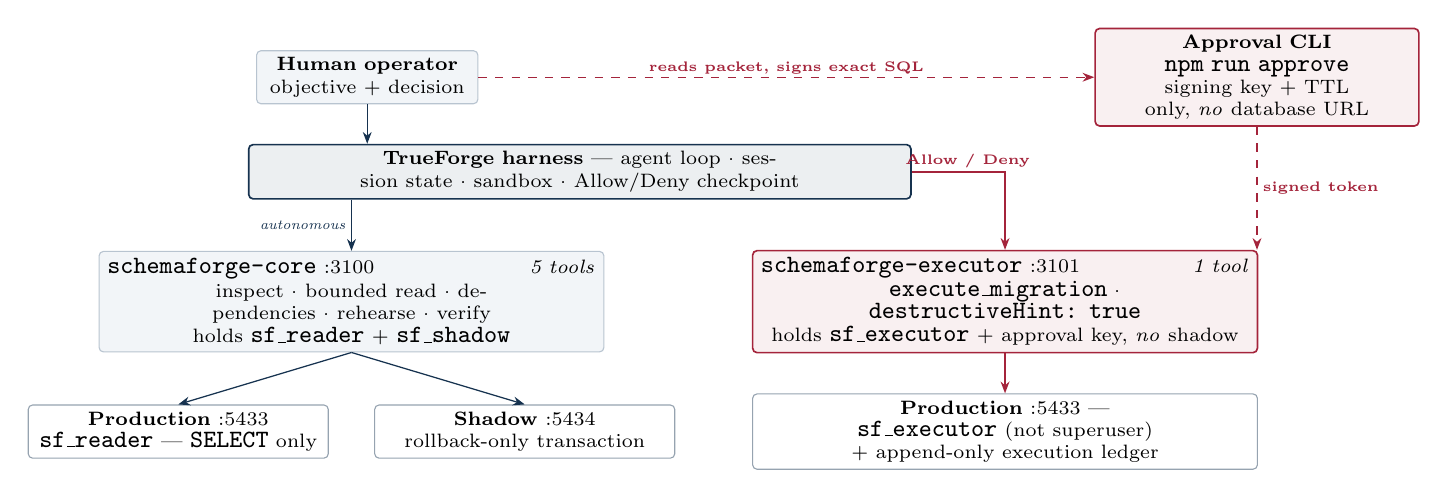
\begin{tikzpicture}
  \node[box, text width=2.6cm] (human) at (2.2,0) {\textbf{Human operator}\\objective + decision};
  \node[danger, text width=3.9cm] (cli) at (13.5,0)
    {\textbf{Approval CLI} \code{npm run approve}\\signing key + TTL only, \emph{no} database URL};

  \node[forge, text width=8.2cm] (forge) at (4.9,-1.2)
    {\textbf{TrueForge harness} --- agent loop \textperiodcentered\ session state \textperiodcentered\ sandbox \textperiodcentered\ Allow/Deny checkpoint};

  \node[box, text width=6.2cm] (core) at (2.0,-2.85)
    {\textbf{\code{schemaforge-core}} :3100 \hfill \emph{5 tools}\\[0.5pt]
     inspect \textperiodcentered\ bounded read \textperiodcentered\ dependencies \textperiodcentered\ rehearse \textperiodcentered\ verify\\[0.5pt]
     holds \code{sf\_reader} + \code{sf\_shadow}};
  \node[danger, text width=6.2cm] (exec) at (10.3,-2.85)
    {\textbf{\code{schemaforge-executor}} :3101 \hfill \emph{1 tool}\\[0.5pt]
     \code{execute\_migration} \textperiodcentered\ \code{destructiveHint: true}\\[0.5pt]
     holds \code{sf\_executor} + approval key, \emph{no} shadow};

  \node[store, text width=3.6cm] (prodro) at (-0.2,-4.5)
    {\textbf{Production} :5433\\\code{sf\_reader} --- \code{SELECT} only};
  \node[store, text width=3.6cm] (shadow) at (4.2,-4.5)
    {\textbf{Shadow} :5434\\rollback-only transaction};
  \node[store, text width=6.2cm] (prodrw) at (10.3,-4.5)
    {\textbf{Production} :5433 --- \code{sf\_executor} (not superuser)\\ + append-only execution ledger};

  \draw[flow] (human) -- (human |- forge.north);
  \draw[token] (human.east) -- node[rlbl, above, pos=0.5] {reads packet, signs exact SQL} (cli.west);
  \draw[flow] (forge.south -| core.north) -- (core.north)
    node[lbl, midway, left=1pt] {autonomous};
  \draw[gated] (forge.east) -| (exec.north)
    node[rlbl, pos=0.3, above] {Allow / Deny};
  \draw[token] (cli.south) -- (cli |- exec.north)
    node[rlbl, midway, right=1pt] {signed token};
  \draw[flow] (core.south) -- (prodro.north);
  \draw[flow] (core.south) -- (shadow.north);
  \draw[gated] (exec.south) -- (prodrw.north);
\end{tikzpicture}
\end{center}

\vspace{-0.6ex}
Both databases run in Docker Compose and are seeded from the \emph{same} deterministic file --- 500 users, exactly 14 NULL emails, a three-row duplicate-email group, boundary foreign keys, precision and zero-quantity edges --- so a shadow rehearsal starts from the fingerprint production actually has. The ledger records every attempt; \code{sf\_executor} may \code{INSERT} and update only four status columns, the nonce is immutable, and migration SQL may not reference the table at all.

\textbf{Correctness mechanics.} Every tool call runs on one physical connection, so \code{BEGIN}, timeouts, work and \code{COMMIT} are never split across pooled sessions. Reads and fingerprints use \code{REPEATABLE READ}, so one hash cannot blend two catalog snapshots. Rehearsal runs inside a transaction that is \emph{only ever rolled back}, with the rollback confirmed rather than assumed and a poisoned connection destroyed instead of reused. Production applies serialize behind an advisory lock under statement and lock timeouts, so a blocked migration fails fast instead of queueing traffic.

\section*{4 \textperiodcentered\ The nine-stage workflow}
Every request walks the same path. Stages 1--7 are autonomous and read-only or sandbox-only; stage 8 is a hard stop; stage 9 exists only after a human acts.

\begin{center}
\nohyph
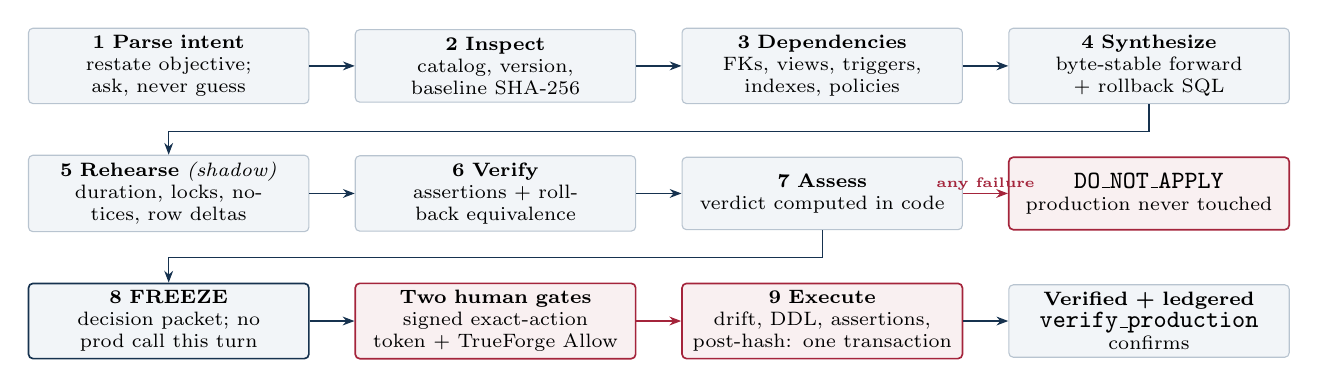
\begin{tikzpicture}[
    stage/.style={box, text width=3.35cm, minimum height=0.92cm},
  ]
  \node[stage] (s1) at (0,0) {\textbf{1 Parse intent}\\restate objective; ask, never guess};
  \node[stage] (s2) at (4.15,0) {\textbf{2 Inspect}\\catalog, version, baseline SHA-256};
  \node[stage] (s3) at (8.3,0) {\textbf{3 Dependencies}\\FKs, views, triggers, indexes, policies};
  \node[stage] (s4) at (12.45,0) {\textbf{4 Synthesize}\\byte-stable forward + rollback SQL};

  \node[stage] (s5) at (0,-1.62) {\textbf{5 Rehearse} \emph{(shadow)}\\duration, locks, notices, row deltas};
  \node[stage] (s6) at (4.15,-1.62) {\textbf{6 Verify}\\assertions + rollback equivalence};
  \node[stage] (s7) at (8.3,-1.62) {\textbf{7 Assess}\\verdict computed in code};
  \node[danger, text width=3.35cm, minimum height=0.92cm] (stop) at (12.45,-1.62)
    {\textbf{\code{DO\_NOT\_APPLY}}\\production never touched};

  \node[stage, draw=sfnavy, line width=0.6pt] (s8) at (0,-3.24)
    {\textbf{8 FREEZE}\\decision packet; no prod call this turn};
  \node[danger, text width=3.35cm, minimum height=0.92cm] (gate) at (4.15,-3.24)
    {\textbf{Two human gates}\\signed exact-action token + TrueForge Allow};
  \node[danger, text width=3.35cm, minimum height=0.92cm] (s9) at (8.3,-3.24)
    {\textbf{9 Execute}\\drift, DDL, assertions, post-hash: one transaction};
  \node[stage] (s10) at (12.45,-3.24) {\textbf{Verified + ledgered}\\\code{verify\_production} confirms};

  \draw[flow] (s1) -- (s2);
  \draw[flow] (s2) -- (s3);
  \draw[flow] (s3) -- (s4);
  \draw[flow] (s4.south) -- ++(0,-0.35) -| (s5.north);
  \draw[flow] (s5) -- (s6);
  \draw[flow] (s6) -- (s7);
  \draw[gated] (s7) -- node[rlbl, above] {any failure} (stop);
  \draw[flow] (s7.south) -- ++(0,-0.35) -| (s8.north);
  \draw[flow] (s8) -- (gate);
  \draw[gated] (gate) -- (s9);
  \draw[flow] (s9) -- (s10);
\end{tikzpicture}
\end{center}

\vspace{-0.4ex}
Evidence is labelled: values returned by a tool are \textbf{[OBSERVED]}; catalog statistics and model inference are \textbf{[ESTIMATED]}. A lock snapshot is never reported as a lock duration.

\textbf{The decision packet} is the artifact the human actually reads, and it has a fixed shape: objective; baseline fingerprint, affected objects and dependency counts; the exact forward and rollback SQL with each statement's transaction class; rehearsal evidence (rehearsal ID, measured duration, lock snapshot, notices, row deltas, and the baseline/post/rollback fingerprints); every named assertion with its actual result; a risk level with its evidence-based factors; and the verdict with rationale. Any field the tools could not produce is written \code{UNAVAILABLE} rather than filled with plausible prose --- an honest inability to prove safety is a reason to stop, not a gap to paper over.


\section*{5 \textperiodcentered\ Where it stops}
The verdict is computed by rule code, not model opinion. The model may explain it; it cannot overturn it.

\begin{tabularx}{\linewidth}{@{}Xl@{}}
\toprule
\textbf{Evidence} & \textbf{Verdict} \\
\midrule
SQL fails policy (prohibited, unsupported, mixed or non-transactional) & rejected before rehearsal \\
Forward SQL fails, or any named assertion fails & \code{DO\_NOT\_APPLY} \\
Rollback ran but did not restore the baseline fingerprint & \code{DO\_NOT\_APPLY} \\
No rollback supplied, or the plan is classified destructive & \code{REVIEW} \\
Rehearsal, assertions and rollback equivalence all verified & \code{APPLY} \\
\bottomrule
\end{tabularx}

\vspace{0.5ex}
A production apply is refused with a distinct machine-readable code, each covered by an automated test:

\begin{tabularx}{\linewidth}{@{}lX@{}}
\toprule
\textbf{Code} & \textbf{Cause} \\
\midrule
\code{SIGNATURE\_INVALID} / \code{TOKEN\_MALFORMED} & Forged, tampered or unparseable approval \\
\code{HASH\_MISMATCH} / \code{ASSERTIONS\_MISMATCH} & SQL or the assertion set edited after the human approved it \\
\code{TOKEN\_EXPIRED} / \code{TOKEN\_NOT\_YET\_VALID} / \code{TTL\_EXCEEDED} & Outside the five-minute window, or an over-long TTL \\
\code{REPLAY\_DETECTED} & Nonce already consumed in the production ledger \\
\code{SCHEMA\_DRIFT} & Production no longer matches the rehearsed baseline \\
\code{POSTCONDITION\_FAILED} & Post-apply fingerprint or an approved assertion failed; transaction rolled back \\
\code{SQL\_POLICY\_REJECTED} & Statement fails the executor's independent policy re-check \\
\bottomrule
\end{tabularx}

\vspace{0.5ex}
Refused unconditionally, even with a valid signature: \code{DROP TABLE}, \code{TRUNCATE}, \code{DROP DATABASE}/\code{SCHEMA}, role and system administration, \code{GRANT}/\code{REVOKE}, \code{COPY ... PROGRAM}, procedural blocks, all DML, any reference to the ledger, and anything outside the canonical fingerprint model. The policy fails \emph{closed}: ambiguous input, such as backslash-escaped literals it cannot lex with certainty, is rejected rather than guessed at.

\section*{6 \textperiodcentered\ How it is used in TrueForge}
TrueForge supplies the agent loop, session state, sandbox and human checkpoints; SchemaForge supplies the tools and the boundary.

\begin{enumerate}
  \item Run the harness (\code{npx @truefoundry/trueforge@0.2.1}) and connect a model under \textbf{Settings $\to$ Models}.
  \item Register two remote MCP connectors: \code{schemaforge-core} at \code{http://127.0.0.1:3100/mcp} and \code{schemaforge-executor} at \code{:3101/mcp}.
  \item Configure a Daytona sandbox provider, used for the agent's own helper code and skills.
  \item Create the agent, pasting \code{trueforge-config/system-prompt.md} into Instructions; \code{agent.yaml} mirrors the remaining fields.
  \item Attach both connectors and require approval for \code{execute\_migration}.
\end{enumerate}

Two independent human boundaries result. TrueForge gates tools the MCP server marks destructive --- its documented default is \code{["@destructive"]}, and the tool is additionally named explicitly --- so the chat pauses on an Allow/Deny card showing the tool and its arguments. Separately, the executor will not act on an Allow alone: it demands the signed token the operator minted in their own terminal after reading the decision packet. Compromising the agent loop is therefore not sufficient to change production. Two prompts make the story visible: asking for \code{users.email} to become \code{NOT NULL UNIQUE} surfaces the 14 NULLs and the duplicate group and ends in \code{DO\_NOT\_APPLY}, production untouched; adding a nullable \code{phone} column rehearses cleanly, proves its rollback, pauses twice, applies atomically, then rejects a replay of the same token.

\section*{7 \textperiodcentered\ Real-world application}
The immediate use is database change management for teams without a dedicated DBA: the agent does the archaeology --- which views, constraints and foreign keys are implicated, how many rows actually violate the new invariant --- and hands over a reviewable packet instead of a diff. It fits naturally as a migration gate in CI/CD, and the ledger doubles as an audit trail: every attempt, approval, rejection code and post-apply fingerprint is recorded in the target database, which is what a regulated environment or a post-incident review asks for.

The transferable part is the pattern, not the SQL. Any domain with cheap analysis and expensive mistakes can reuse it: rehearse in a disposable copy, gather measured evidence, compute the verdict in code, bind a short-lived signed approval to one exact action, verify postconditions inside the same transaction, and record the outcome. Cloud teardown, access revocation, release publishing and infrastructure runbooks share that shape --- the agent is trusted to investigate, never to decide.

\section*{8 \textperiodcentered\ Known limitations}
Stated plainly, because a safety tool that overstates its reach is the problem it claims to solve.

\begin{multicols}{2}
\begin{itemize}
  \item \textbf{PostgreSQL and the \code{public} schema only.} One database per target; no MySQL, no cross-schema or cross-database migrations.
  \item \textbf{Transactional schema DDL only.} \code{CREATE INDEX CONCURRENTLY}, \code{REINDEX CONCURRENTLY} and \code{VACUUM} cannot be made atomic, so they are refused rather than pretended to be reversible; they need a separately designed recovery workflow.
  \item \textbf{No data migrations.} All DML is rejected. Backfills, deduplication and the remediation that would make the \code{NOT NULL} example succeed are out of scope --- the executor proves schema state, not data equivalence.
  \item \textbf{The fingerprint defines the frontier.} It covers tables, columns with full type modifiers, constraints, indexes, views and extensions. What it cannot represent --- function bodies, trigger state, ownership, partition topology, storage parameters --- is excluded from the allowlist rather than silently unverified.
  \item \textbf{The SQL policy is a conservative lexer with an allowlist, not a complete PostgreSQL parser.} It is designed to under-approximate: the database's own least-privilege roles remain the backstop.
  \item \textbf{Rehearsal measures a seeded copy, not production scale.} Timings and lock observations are directionally useful, not capacity planning, and the lock reading is a point-in-time snapshot.
  \item \textbf{Local, single-tenant scope.} One approval key, one target, no multi-tenant routing; the bundled credentials are demo values for a local Compose stack, and the harness itself runs in TrueForge's localhost mode.
  \item \textbf{Verification status.} Types, build, 32 security unit tests and 7 live MCP transport/boot tests pass locally; the 25 PostgreSQL scenarios run in CI against fresh PostgreSQL~16 containers, and were skipped on the authoring machine because Docker was not running.
\end{itemize}
\end{multicols}

\vfill
{\color{sfrule}\hrule height 0.4pt}
\vspace{0.5ex}
{\footnotesize Repository: \url{https://github.com/harshaxyZ/schemaforge} \textperiodcentered\ MIT licence \textperiodcentered\ Validate with
\code{npm run check}, \code{npm run build}, \code{npm test} \textperiodcentered\ Built with AI assistance (Claude Opus 5);
the human team owns the architecture and product decisions.}

\end{document}
